\section{Getting Started}

The examples in this document refer to a \gtis{LINUX} machine, however, they
should be easy to understand and adapted to a \gtis{WINDOWS} computer.

The main differences are, that the slashes in the file and path names must
be replaced by backslashes, shell scripts ($*.sh$) must be replaced
by  $*.bat$ files, and the system variables $\$V$ must be
replaced by $\%V\%$.

\subsection{Running WAVE}

Under \gtis{WINDOWS} open e.g. a DOS command shell (cmd.exe), goto to
the directory where \W is installed and excute
\gtis{bat\textbackslash set\_wave\_environment.bat}\bsp. Then enter
\gtis{wave} or \gtise{waveshop}. But as mentioned before, we now refer to \gtise{LINUX}.

First define a shell variable \dw~ containing the path to your
\W-directory:

~~~~~\gtise{export WAVE=YOUR-WAVE-DIRECTORY}

~~~~~\gtise{export WAVE\_INCL=\dw}

It is recommended to put these lines in a script, see e.g.

~~~~~\senv

and to excute it at the beginning of a \W-session.

To run \W the traditional way is to is to enter in a terminal

~~~~~\gtis{cd \dw/bin/stage}

~~~~~\gtis{../bin/wave.exe}\\

It is recommended to use the script

~~~~~\gtis{\dw/stage/wave}

to run \W.

WAVE should run and write some output to your terminal (Fig.~\ref{gsfig3}).

\begin{figure}[htb]
    \centering
    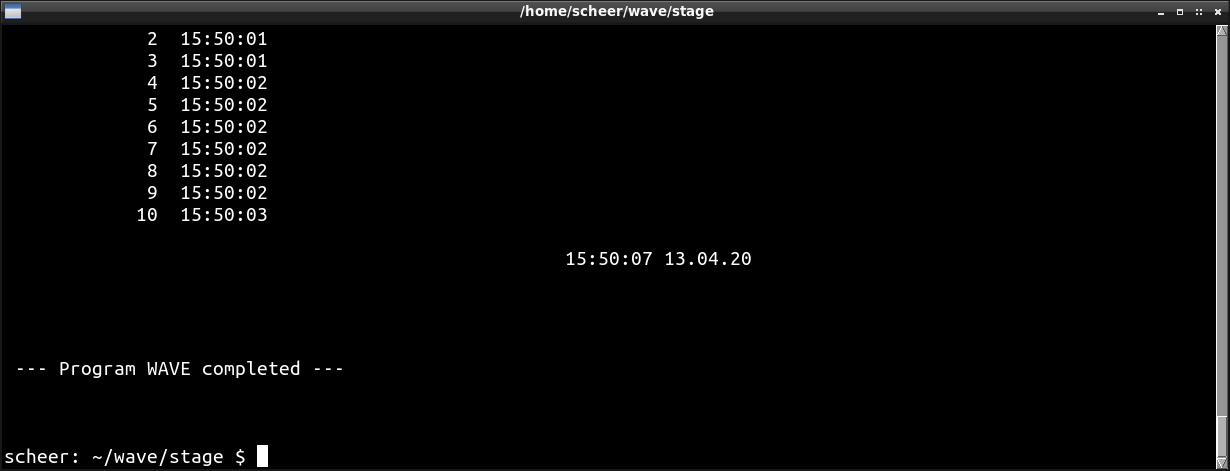
\includegraphics[width=0.75\textwidth]{pics/wave_run.png}
    \caption{Terminal output of \textit{WAVE}}
    \label{gsfig3}
\end{figure}

The program writes some output to the screen and the output text files
\wo and
\mhbe. The file \wo contains the most important
in- and output of the run, while \mhb contains the histograms and
n-tuples to be plotted. Please open these files and have a look{\ldots}

If the program crashes, it must probably be recompiled in your
environment by

~~~~~\gtis{python3 \dw/python/make\_wave.py}

if you have \gtis{gfortran} installed, or by

~~~~~\gtis{python3 \dw/python/make\_wave\_intel.py}

if you have the Intel compiler \gtis{ifx} installed.

If these Python scripts are run with an argument, they run in a verbose mode.

\subsection{Plotting with Python}

A convenient way to visualize the histograms and
n-tuples is to use a Python scripts

~~~~~\gtis{python3 -i ../python/waveplot.py}

First, we check the installation of Python. Enter:

~~~~~\gtis{python3}

If you get a \gtis{Python} command prompt, \gtis{Python3} is
installed. Note: Under \gtis{WINDOWS} the command is probably
\gtis{python} instead of \gtis{python3}. However, the version $3.x$ of {\it
Python} is required. You can leave the \gtis{Python} shell with:

~~~~~\gtis{quit()}

If the test was successful, try the same with ipython3:

~~~~~\gtis{ipython3}

If there is no command \gtis{ipython3}, you can install it (given pip3
is installed):

~~~~~\gtis{pip3 install ipython3}

\subsection{The Graphical User Interface \WSH}

There is a graphical user interfaces (GUI) based on \gtis{Python} and
\gtis{Tkinter}.

To run the GUI \WSH (Fig.~\ref{gsfig1}), you need \gtis{python3} or
\gtie{ipython3}. In addition,
the file \gtis{waves.wvs} must be present in the
working directory. The \gtis{Python} script \gtis{../python/waveshop.py} is started by
the command alias \gtis{waveshop}. Thus enter

~~~~~\WSH

or, if the alias is not defined accordingly, by

~~~~~\gtis{python3 -i ../python/waveshop.py}

\begin{figure}[t]
    \centering
    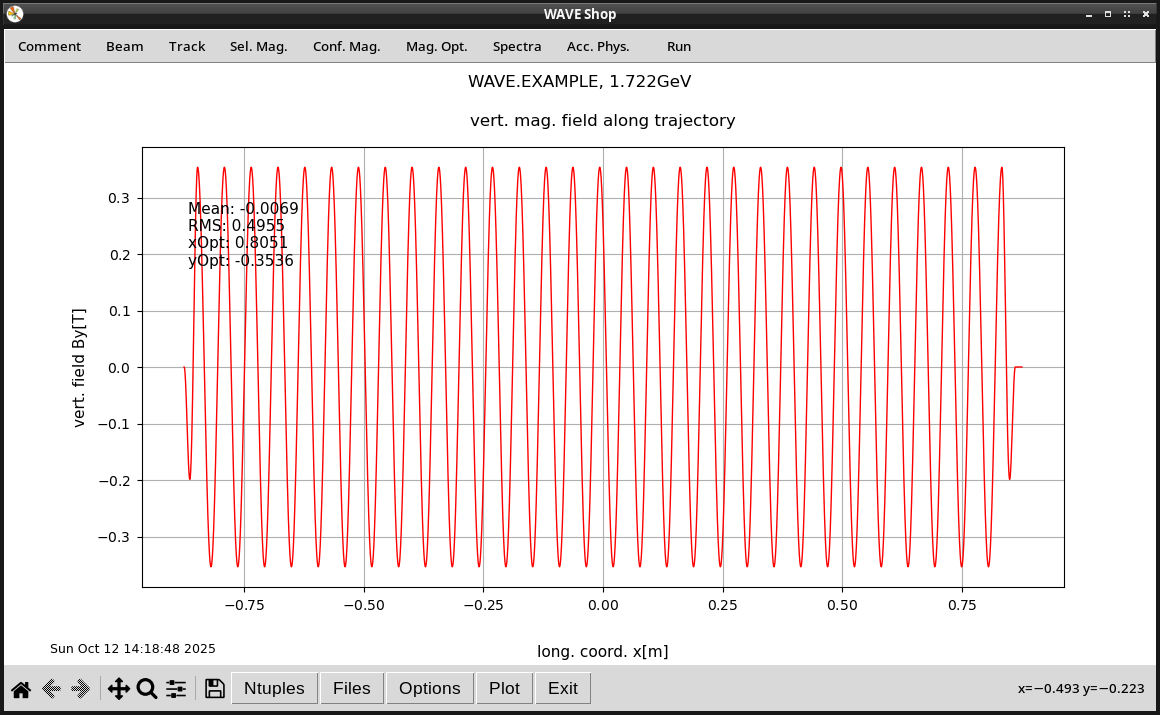
\includegraphics[width=0.95\textwidth]{pics/waveshop_gsfig1.png}
    \caption{Main window of \WSH. The upper menu items
    are used to set-up \wi and to run \W, the lower buttons to plot the
    results.}
    \label{gsfig1}
\end{figure}

%\newpage
\subsection{The Input File \gti{wave.in}}

The GUI for \W covers many standard calculations, however,
to get the most out of \W, it is necessary to study and
understand the input file \wie.

\begin{figure}[htb]
    \centering
    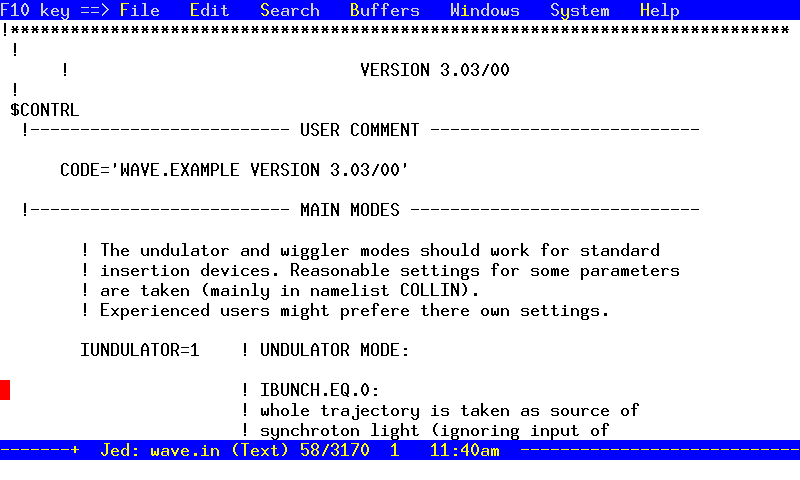
\includegraphics[width=0.7\textwidth]{pics/ex1_wave_in.png}
    \caption{First part of the input file \textit{wave.in}}
    \label{gsfig6}
\end{figure}

We open \wi with an editor and search \contrl. This keyword
belongs to a \gtis{FORTRAN} namelist. A namelist begins with such a keyword
and ends with \dend. The file \wi is actually nothing than a list of
namelists.

A namelist is a list of variables, read by the program. The position
of the variable in the namelist does'nt matter. Missing variables are
initiliazed as zero or an empty string. For the name of the variables
the \gtis{FORTRAN} conventions aplly, i.e. variables beginning with \gtis{I, J, K,
L, M, N} are integer, all others are strings, floating point, or complexe
numbers. The integer must not have a decimal point, while the floating
point  and complexe numbers onces must have. The same
variable may occur several times within a namelist. Then the last
value is accepted. If a whole namelist occurs several times, only the
first one is read. Comments must begin with~"!".

The namelist \contrl is the most important one of \wie. It
controlls the program flow, the tracking, the field selection and so on.

\newpage
A short example: Look for a line, containing

\cboxs{KELLIP=1}

This variables activates an analytical model of an elliptical
undulator. The comment in this line mentions the namelist \scap{\$ELLIPN}.
Hence, we search \scap{\$ELLIPN}.

\begin{figure}[htb]
    \centering
    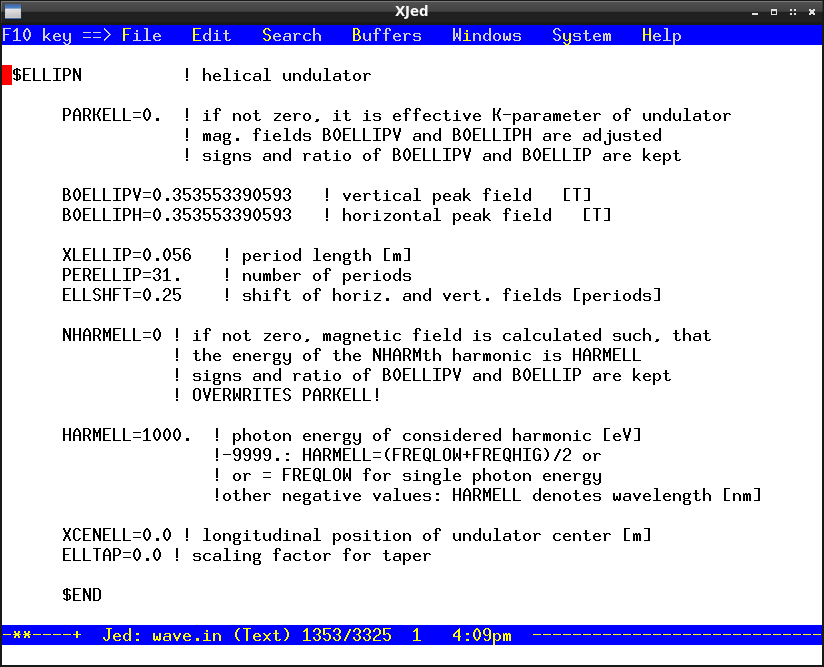
\includegraphics[width=0.7\textwidth]{pics/ellipn.png}
    \caption{The namelist \gtis{ELLIPN} of
    the elliptcal undulator model}
    \label{gsfig7}
\end{figure}

\newpage
Here you could change the parameters of the selected elliptical
undulator.

\ul{Note}: The GUI \WSH can't handle multiple occurances of
variables, i.e. it always takes the first value. So it's better to
avoid it. If you want to keep a copy of an old value, change the line
into a comment line.

Editing input files might appear a little old-fashioned today, but has
the big advantage of easy documentation and allows to run and control
the program from scripts, which can be very effective e.g in
optimization procedures.

\renewcommand*\thesection{\arabic{section}. \hspace{-4mm}}
\setcounter{section}{0}
